% CVPR 2026 Paper Template; see https://github.com/cvpr-org/author-kit
\documentclass[10pt,twocolumn,letterpaper]{article}

% Page numbers are useful while the assignment report is being assembled.
\usepackage[pagenumbers]{cvpr}

\usepackage{graphicx}
\usepackage{amsmath}
\usepackage{amssymb}
\usepackage{booktabs}
\usepackage{array}
\usepackage{multirow}
\usepackage{microtype}
\usepackage{xcolor}
\usepackage{xspace}
\usepackage{enumitem}
\usepackage{url}

\newcommand{\method}{RGB-DP\xspace}
\newcommand{\successonce}{\texttt{success\_once}\xspace}
\newcommand{\successend}{\texttt{success\_at\_end}\xspace}
\newcolumntype{R}[1]{>{\raggedleft\arraybackslash}p{#1}}

% T-I final-evaluation values. Keeping them centralized prevents numerical drift
% between the abstract, table, discussion, and conclusion.
\newcommand{\tiseedzero}{12\%}
\newcommand{\tiseedone}{13\%}
\newcommand{\tiseedtwo}{8\%}
\newcommand{\tiseedzeroend}{11\%}
\newcommand{\tiseedoneend}{13\%}
\newcommand{\tiseedtwoend}{8\%}
\newcommand{\tiseedzeromax}{0.545}
\newcommand{\tiseedonemax}{0.518}
\newcommand{\tiseedtwomax}{0.494}
\newcommand{\tiseedzerofinal}{0.429}
\newcommand{\tiseedonefinal}{0.413}
\newcommand{\tiseedtwofinal}{0.385}
\newcommand{\timean}{11.0}
\newcommand{\tistd}{2.65}
\newcommand{\tipooled}{33/300}
\newcommand{\timeanend}{10.7}
\newcommand{\tistdend}{2.52}

\setlist[itemize]{leftmargin=*,nosep}
\setlist[enumerate]{leftmargin=*,nosep}


\definecolor{cvprblue}{rgb}{0.21,0.49,0.74}
\usepackage[pagebackref,breaklinks,colorlinks,allcolors=cvprblue]{hyperref}

\def\paperID{RIPL-Assignment}
\def\confName{CVPR}
\def\confYear{2026}

\title{Visual Diffusion Policy on ManiSkill Push-T:\
Training, Failure-Analysis Protocol, and Proposed Residual Learning}

\author{Renana Kashima\\
RIPL Lab Prospective Student Assignment}

\begin{document}
\maketitle

\begin{abstract}
We implement and train an RGB-conditioned Diffusion Policy for ManiSkill's
\texttt{PushT-v1} task. The reportable experiment uses 100 successful, controller-native
demonstrations replayed with temporally aligned RGB observations, two observation frames, a
16-step prediction horizon, one-step receding-horizon execution, and 50,000 optimization steps.
The selected EMA checkpoint is fixed at iteration 15,000, where a 20-episode diagnostic first
reaches 30\% \successonce. On the required independent evaluation of 100 rollouts at each of
three environment seeds, it obtains \textbf{\timean\% $\pm$ \tistd{} percentage points}
(\tipooled{} pooled successes).

The 1,000-step moving-average diffusion loss decreases from 0.0533 at iteration 11,000 to 0.0183
at 50,000. The preserved Runpod continuation from 10,000 to 50,000 takes 2 h 19 min 2 s across
two restart-safe segments; the uninterrupted 15,000--50,000 segment takes 2 h 2 min 35 s on one
NVIDIA A40 and peaks at 7,603 MiB (7.42 GiB) sampled VRAM. We also document the principal
debugging result: an earlier GPU replay paired actions with a one-step-shifted environment state.
Correcting the replay to restore $s_{t+1}$ after action $a_t$, matching the original 1,024-way
simulation parallelism, and retraining from a valid checkpoint transformed a zero-success
pipeline into a measurable Push-T baseline. The final result remains limited by one training
seed and a noisy checkpoint-selection diagnostic; these limitations motivate the targeted
failure analysis in T-II. T-II tooling for pose-conditioned resets, trajectory capture, and
failure screening was implemented and tested, but the required discovery and targeted rollout
experiments did not complete because replacement GPU instances either lacked a working Vulkan
graphics path or were unavailable. Consequently, this report does not claim two validated failure
modes, targeted success rates, or representative T-II videos. T-III and T-IV were also not
completed; we instead state the intended LLM reward-generation and bounded residual-PPO methods,
including the validation needed to avoid reward hacking and distributional regressions.
\end{abstract}

\section{Introduction}

T-I asks for a visual-input Diffusion Policy trained by imitation learning in ManiSkill, together
with training loss, hyperparameters, resource use, and a fixed-checkpoint evaluation over 100
rollouts at three random seeds. We choose \texttt{PushT-v1}, a contact-rich planar manipulation
task in which the robot must push a T-shaped block into a fixed T-shaped goal. This policy also
serves as the base policy whose reproducible failures are studied in T-II--T-IV.

Diffusion Policy represents visuomotor control as conditional denoising over action
sequences~\cite{chi2023diffusion}. ManiSkill provides the task, GPU-parallel simulator,
demonstrations, wrappers, and reference implementation used here~\cite{tao2024maniskill3,
maniskill_baseline}. We first implemented the official quick-start exercises to verify scene
creation, batched environment reset and stepping, RGB rendering, controllers, and task metrics,
then adapted ManiSkill's Diffusion Policy baseline into a standalone Python
package~\cite{maniskill_quickstart}.

The main empirical and engineering findings are:
\begin{itemize}
    \item A spatial RGB Diffusion Policy trained on 100 aligned demonstrations produces a
    nonzero Push-T baseline under a fixed 300-rollout evaluation.
    \item Diffusion loss falls steadily, but lower loss does not imply a better closed-loop
    checkpoint: 20-episode diagnostic success fluctuates from 10\% to 30\% after iteration 15k.
    \item The best checkpoint is iteration 15k. Iteration 40k ties its 30\% diagnostic score, but
    strict-improvement selection correctly retains the first maximum.
    \item The decisive roadblock was data alignment, not merely model capacity. The initial RGB
    replay restored $s_t$ after executing $a_t$; the corrected pipeline restores $s_{t+1}$ and
    validates every trajectory before training.
    \item Checkpoint-complete resumption across interrupted GPU sessions preserves optimizer,
    scheduler, EMA, iteration, and checkpoint-selection state, permitting an auditable 50k run.
\end{itemize}

As a debugging control, the same visual pipeline previously reached 82.0\% $\pm$ 4.6 percentage
points on \texttt{PushCube-v1}. That result established that RGB replay, spatial encoding,
denoising, and closed-loop evaluation functioned end to end; it is not substituted for the
requested Push-T result in this report.

\section{Method}

\subsection{Task, observations, and actions}

Push-T fixes the goal at world position $(-0.156,-0.100)$ m with yaw $300^\circ$ and samples the
T block across position and orientation~\cite{maniskill_pusht}. Success requires the rendered
intersection between the block and goal to reach at least 0.90. The primary metric,
\successonce, records whether this threshold is reached at any point; \successend records whether
it remains satisfied at the time limit.

The policy receives RGB images and robot proprioception, but no privileged block or goal pose. At
each decision it conditions on observation horizon $T_o=2$. RGB frames are scaled to $[0,1]$ and
processed by a five-layer convolutional encoder. A $128\!\times\!128$ image becomes a
$128\!\times\!8\!\times\!8$ feature map, which is flattened and projected to 256 dimensions.
Retaining this spatial map is important because global pooling discards absolute block and goal
location. The visual feature is concatenated with robot state at each observation step.

The demonstrations and evaluation both use ManiSkill's \texttt{pd\_ee\_delta\_pose} controller.
Actions are normalized to $[-1,1]$. We execute one action and immediately replan
($T_a=1$), matching the tuned Push-T control pattern and limiting open-loop error during contact.

\subsection{Conditional action diffusion}

The policy predicts noise for a $T_p=16$ action sequence with a conditional one-dimensional
U-Net. It uses channel widths $[64,128,256]$, GroupNorm, Mish activations, skip connections, and
FiLM-style conditioning on visual-proprioceptive history and a 64-dimensional sinusoidal
diffusion-step embedding. Training samples diffusion step $k$, adds noise $\epsilon$ to a
demonstrated action sequence, and minimizes
\begin{equation}
    \mathcal{L}(\theta)=
    \mathbb{E}_{a,\epsilon,k}\!
    \left[\left\|\epsilon-\epsilon_\theta(a_k,k,o_{t-1:t})\right\|_2^2\right].
\end{equation}
We use 100 denoising steps and a squared-cosine DDPM schedule~\cite{nichol2021improved}.

\subsection{Aligned RGB demonstration replay}
\label{sec:aligned-replay}

The downloaded RL demonstrations contain simulator states rather than the required RGB sequence.
We replay the first 100 successful \texttt{pd\_ee\_delta\_pose} trajectories with
\texttt{physx\_cuda}, RGB observations, and the original 1,024 parallel environments. The
validated dataset contains 9,865 transitions and 9,765 training windows.

A trajectory with $T$ actions contains $T+1$ environment states. After action $a_t$, the
observation paired with the next action must begin at $s_{t+1}$. The audited upstream replay path
restored $s_t$ instead; our fail-closed wrapper changes this operation to
\texttt{env\_states[t + 1]} in process and rejects source code that does not match the audited
pattern. Before training, the validator checks source success labels, controller, collection and
replay parallelism, output observation mode, trajectory count, and exactly $T+1$ RGB observations
for $T$ actions in every episode.

\subsection{Training and checkpoint protocol}

We train one model with seed 1 using AdamW, batch size 128, learning rate $10^{-4}$, 500 linear
warmup steps, and cosine decay. Demonstration tensors remain on CPU and minibatches are transferred
to the GPU. EMA weights with power 0.75 are used for rollout evaluation. Training runs for 50,000
updates; loss is logged every 100 updates, and a checkpoint is saved every 5,000.

Every 5,000 updates, 20 fresh episodes provide a model-selection diagnostic. A checkpoint replaces
\texttt{best\_success\_once.pt} only when \successonce strictly improves. Interrupted sessions
resume the complete training state, not just model weights. The run begins from a 10k Colab
checkpoint, continues to 15k, and resumes from the validated 15k checkpoint to 50k on Runpod.

\subsection{Fixed-checkpoint evaluation}

Final evaluation loads the single selected EMA checkpoint and runs 100 fresh episodes for each
environment seed in $\{0,1,2\}$. All seeds use the same training checkpoint; they are not three
independently trained policies. The evaluator reconfigures every environment, ignores early task
termination until the 150-step limit, and records synchronized complete episodes. We report each
seed, the arithmetic mean and sample standard deviation of the three success rates, and pooled
successes out of 300. Auxiliary metrics include return, maximum overlap, final overlap, and
\successend.

\section{T-I: Push-T Results}

\subsection{Configuration}

Table~\ref{tab:pusht-config} records the resolved configuration used by the reportable run. It is
saved with the checkpoints rather than reconstructed from command history.

\begin{table}[t]
    \centering
    \caption{Reportable Push-T training configuration.}
    \label{tab:pusht-config}
    \footnotesize
    \begin{tabular}{@{}p{0.62\linewidth}R{0.29\linewidth}@{}}
        \toprule
        Setting & Value \\
        \midrule
        Training seed / RGB demonstrations & 1 / 100 \\
        Transitions / windows & 9,865 / 9,765 \\
        Observation / action / prediction horizon & 2 / 1 / 16 \\
        Diffusion steps & 100 \\
        U-Net widths & $[64,128,256]$ \\
        Spatial visual feature dimension & 256 \\
        Batch size / learning rate & 128 / $10^{-4}$ \\
        Warmup / total updates & 500 / 50,000 \\
        Maximum episode steps & 150 \\
        Backend / controller & GPU PhysX / delta pose \\
        Dataset device / policy device & CPU / CUDA \\
        \bottomrule
    \end{tabular}
\end{table}

\subsection{Training dynamics and checkpoint selection}

Figure~\ref{fig:pusht-results} summarizes the optimization and evaluation evidence. The
1,000-step moving-average diffusion loss decreases from 0.0533 at iteration 11k to 0.0183 at 50k.
The raw logged loss at 50k is 0.0274. This establishes optimization progress, but it does not
identify the best controller: diagnostic \successonce peaks at 30\% at 15k, drops to 10\% at
25k, and returns to 30\% at 40k even as loss continues to decrease.

The selected checkpoint is therefore the EMA policy at iteration 15k. The 40k score ties rather
than exceeds the first maximum, and the implementation intentionally requires strict improvement.
This avoids silently changing a selected checkpoint on an equal, noisy 20-episode estimate.

\begin{figure*}[t]
    \centering
    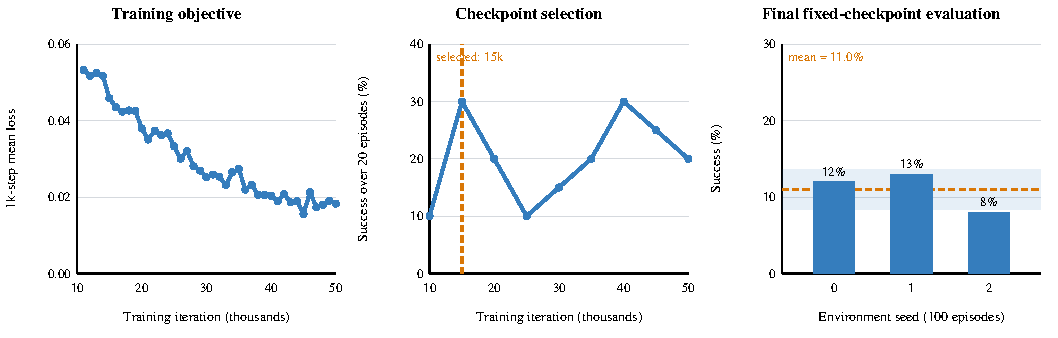
\includegraphics[width=0.99\textwidth]{fig/pusht_ti_results.pdf}
    \caption{\textbf{Left:} diffusion loss logged every 100 updates and summarized by a trailing
    1,000-step mean. The original 0--10k Colab event file was not preserved, so the trace begins at
    10.1k. \textbf{Center:} 20-episode \successonce diagnostic used only for checkpoint selection;
    the dashed marker is the selected 15k checkpoint. \textbf{Right:} reportable evaluation of
    that fixed checkpoint over 100 fresh rollouts per seed. The line and band denote the
    three-seed mean and one sample standard deviation.}
    \label{fig:pusht-results}
\end{figure*}

\subsection{Fixed-checkpoint baseline}

Table~\ref{tab:pusht-eval} reports the required 300-rollout evaluation. The fixed 15k checkpoint
achieves \tiseedzero, \tiseedone, and \tiseedtwo{} \successonce for seeds 0, 1, and 2. The
three-seed baseline is \textbf{\timean\% $\pm$ \tistd{} percentage points}, with \tipooled{}
pooled successes. The corresponding mean \successend is \timeanend\%.

\begin{table}[t]
    \centering
    \caption{Fixed 15k checkpoint; 100 Push-T rollouts per environment seed.}
    \label{tab:pusht-eval}
    \footnotesize
    \setlength{\tabcolsep}{4pt}
    \begin{tabular}{@{}lrrrr@{}}
        \toprule
        Seed & Once & End & Max ov. & Final ov. \\
        \midrule
        0 & \tiseedzero & \tiseedzeroend & \tiseedzeromax & \tiseedzerofinal \\
        1 & \tiseedone & \tiseedoneend & \tiseedonemax & \tiseedonefinal \\
        2 & \tiseedtwo & \tiseedtwoend & \tiseedtwomax & \tiseedtwofinal \\
        \midrule
        Mean & \timean\% & \timeanend\% & -- & -- \\
        Sample std. & \tistd{} pp & \tistdend{} pp & -- & -- \\
        \bottomrule
    \end{tabular}
\end{table}

The final estimate is lower than the 30\% selection diagnostic. This is not a contradiction: the
diagnostic contains only 20 episodes and was repeatedly queried during training, while each final
seed contains 100 fresh episodes. The larger evaluation is the baseline; the diagnostic is only a
checkpoint-selection instrument. A nonzero gap between \successonce and \successend also captures
policies that reach 0.90 overlap transiently and subsequently displace the block.

\subsection{Training time and resource use}

The first 10,000 updates were trained in Colab, but the Colab start timestamp was not preserved;
we therefore do not invent an end-to-end wall time. The measured Runpod continuation from 10k to
15k takes 16 min 27 s including its diagnostic evaluation. After a process termination, the
checkpoint-complete 15k--50k continuation takes 2 h 2 min 35 s, also including seven scheduled
20-episode evaluations. The total observed 10k--50k continuation is 2 h 19 min 2 s.

For the uninterrupted 15k--50k segment, \texttt{nvidia-smi} was sampled every 5 s for 1,475
measurements. On one 46,068 MiB NVIDIA A40, peak sampled allocation is 7,603 MiB (7.42 GiB), peak
sampled utilization is 54\%, and peak sampled power is 187.93 W. ``Sampled'' is essential: these
are observations at discrete times, not guaranteed instantaneous maxima.

\section{T-I Debugging and T-II Status}
\label{sec:debugging}

\subsection{Why the first Push-T run was rejected}

An earlier spatial RGB checkpoint reached 0\% closed-loop success despite low offline diffusion
loss, high cosine similarity to stored demonstration actions, and strong sensitivity to shuffled
RGB. Those diagnostics showed that the model fit its dataset; they did not establish that the
dataset represented the intended observation-action relation. Treating that checkpoint as a valid
base policy would have made every downstream failure frequency scientifically ambiguous.

The replay audit identified a concrete temporal defect. In a state-restored trajectory, action
$a_t$ advances the simulator from $s_t$ to $s_{t+1}$. The subsequent rendered observation must
therefore correspond to $s_{t+1}$. The original GPU replay restored $s_t$ after the action,
creating a shifted supervised mapping while preserving plausible images and valid tensor shapes.
Section~\ref{sec:aligned-replay} describes the fail-closed correction and validation gates. The
pre-fix checkpoint was not resumed because changing the dataset changes the learned conditional
mapping.

\noindent\textbf{Fail-closed alignment patch (abridged).}
\begin{minipage}{\linewidth}
\scriptsize
\begin{verbatim}
OLD = "set_state_dict(env_states_batch[t])"
NEW = "set_state_dict(env_states_batch[t + 1])"
if source.count(OLD) != 1:
    raise RuntimeError("inspect installed source")
source = source.replace(OLD, NEW)
\end{verbatim}
\end{minipage}

\subsection{Controls and independent troubleshooting}

Several controls separated data, architecture, and infrastructure failures. First, a spatial
feature encoder replaced global visual pooling because Push-T withholds privileged object and goal
pose; absolute image location is therefore task-relevant. Second, an RGB PushCube control reached
82.0\% $\pm$ 4.6 percentage points over 300 rollouts, validating the common image replay, policy,
EMA, and evaluator. Third, the corrected Push-T replay matched the source controller and original
1,024-environment collection parallelism rather than changing several variables simultaneously.

Infrastructure problems were also made explicit rather than hidden. Python 3.12 and headless
Vulkan were verified before training. HCE jobs call Python directly because nesting \texttt{srun}
inside the allocation caused CPU-binding failures. Runpod training was detached from SSH, logged
to persistent storage, checkpointed every 5k, and resumed from the newest validated checkpoint
after termination. These decisions are part of reproducibility, not incidental operational detail.

\subsection{Limitations and hidden assumptions}

The result supports a trained visual Push-T baseline, but it does not establish robustness:
\begin{itemize}
    \item Only one policy-training seed (seed 1) was affordable. The reported standard deviation
    measures environment-seed variation for one fixed policy, not training-seed variability.
    \item Checkpoint selection repeatedly evaluates 20 episodes. Its maximum is statistically
    noisy and selection-biased, as demonstrated by the lower 300-rollout estimate.
    \item Push-T GPU replay is sensitive to collection parallelism and simulator state restoration.
    Matching 1,024 environments reduces a known discrepancy but does not prove bitwise equivalence
    across hardware or ManiSkill versions.
    \item \successonce is the official baseline metric, but it credits transient goal entry. We
    retain \successend, maximum overlap, final overlap, and videos to expose this distinction.
    \item The loss trace starts at 10.1k because the original Colab TensorBoard event file was not
    preserved. Checkpoints and evaluation metrics from that segment remain available.
\end{itemize}

These caveats motivate T-II's pose-conditioned evaluation: aggregate success alone cannot reveal
which initial configurations fail, whether distinct mechanisms are reproducible, or whether a
later residual policy improves targeted failures without harming nominal behavior.

\subsection{T-II: implemented protocol, incomplete experiments}

T-II was not completed. We implemented a separate \texttt{t-ii/} package that samples exact
subsets of Push-T's nominal initial-pose domain, records the initial T pose and TCP pose, saves
per-step overlap trajectories, assigns non-exclusive screening tags, and aggregates success with
Wilson intervals. Unit tests cover wrapped angular ranges, exact pose-conditioned resets, metric
serialization, and failure-tag logic. These tests establish the evaluation machinery, not two
empirical failure modes.

The preregistered discovery protocol was 200 full-distribution rollouts from relative block
position $x\in[-0.10,0.10]$ m, $y\in[-0.10,0.20]$ m and yaw $\theta\in[0,360)^\circ$. Candidate
regions would be selected only after jointly inspecting initial-pose bins, overlap trajectories,
and videos. Two useful screening hypotheses were (i) low progress after loss of contact and
(ii) progress regression after transient partial or successful goal overlap. These are plausible
mechanisms, not reported findings. Each accepted mode would then require a representative MP4 and
100 targeted rollouts at each seed in $\{0,1,2\}$.

The valid visual run could not be executed before the deadline. The original A40 completed T-I
and was safely backed up. A replacement A100 booted and received the hash-verified checkpoint, but
RGB environment creation failed with \texttt{vk::createInstanceUnique:
ErrorIncompatibleDriver}; graphics-capable A40, RTX A6000/4090, RTX 4000 Ada, and L4 instances
were unavailable. A local Apple M4 smoke test reproduced the missing-Vulkan barrier. We rejected
a state-only substitute because it would not evaluate the trained RGB policy. Thus there are no
defensible T-II per-mode rates or videos, and none are fabricated or inferred from T-I diagnostic
rollouts.

We also avoid treating an external number as a required target. ManiSkill issue \#882 reports one
state-input reproduction near 0.15--0.20 and asks why a paper reports 0.4--0.5, but it does not
establish an expected RGB result or resolve differences in data and simulation
settings~\cite{maniskill_issue882}. Our baseline is therefore defined by its disclosed protocol,
not by post-hoc agreement with that thread.

\section{Engineering and Reproducibility}

The project targets Python 3.10--3.12 and separates configuration, data, networks, policy,
environment construction, and evaluation into testable modules. YAML defines the experiment, and
the resolved JSON configuration is copied into every run directory. Checkpoints contain online and
EMA weights, optimizer and scheduler state, EMA state, current iteration, best metrics, and the
training configuration. This is why the 15k continuation is mathematically the same scheduled run
rather than an informal warm start.

The measured environment is summarized in Table~\ref{tab:software}. The Pod used the mutable
\texttt{maniskill/base:latest} image, so exact package versions are recorded to remove ambiguity.

\begin{table}[t]
    \centering
    \caption{Software and hardware for the completed Push-T run.}
    \label{tab:software}
    \footnotesize
    \begin{tabular}{@{}ll@{}}
        \toprule
        Component & Version / device \\
        \midrule
        Python / ManiSkill / SAPIEN & 3.12.13 / 3.0.1 / 3.0.3 \\
        PyTorch / Diffusers & 2.13.0 / 0.40.0 \\
        Gymnasium / NumPy / h5py & 1.3.0 / 2.5.2 / 3.16.0 \\
        GPU / driver-reported CUDA & NVIDIA A40 / 13.0 \\
        \bottomrule
    \end{tabular}
\end{table}

The evaluator writes one \texttt{metrics.json} per seed, and a separate aggregation command writes
\texttt{summary.json}. Complete evidence includes the aligned HDF5 and metadata hashes, config,
checkpoint lineage, both training logs, TensorBoard events, five-second GPU CSV, seed metrics,
aggregate summary, and videos. Large artifacts are backed up outside ordinary Git history; source,
configs, tests, launchers, and concise result summaries remain in Git.

Implementation safeguards include:
\begin{itemize}
    \item CPU vector environments expose episode metrics directly, whereas the GPU wrapper may
    place them under \texttt{final\_info}; the evaluator supports both representations.
    \item Underscore-prefixed fields such as \texttt{\_success\_once} are Gymnasium validity masks,
    not metrics. Aggregation uses the corresponding non-prefixed value.
    \item All evaluation environments use \texttt{reconfiguration\_freq=1}; otherwise cached scene
    configurations can make nominally different episodes share initialization state.
    \item RGB replay aborts on controller, parallelism, observation-count, or source-code mismatch
    instead of silently producing a different dataset.
    \item Unit tests cover configuration validation, temporal sequence construction, policy shapes,
    CPU/GPU metric extraction, three-seed aggregation, replay alignment, and dataset provenance.
\end{itemize}

The local verification suite contains 20 passing T-I tests. The repository exposes equivalent
Colab, HCE, and Runpod entry points, but the minimal reproduction path is the stage-based Runpod
launcher in Appendix~\ref{sec:reproduction}.

\section{T-III and T-IV: Proposed Approaches}

Table~\ref{tab:status} separates completed evidence from proposed work. ``Not completed'' means
that no empirical result is claimed.

\begin{table}[t]
    \centering
    \caption{Assignment status at submission time.}
    \label{tab:status}
    \footnotesize
    \begin{tabular}{@{}p{0.13\linewidth}p{0.22\linewidth}p{0.53\linewidth}@{}}
        \toprule
        Stage & Status & Evidence / next gate \\
        \midrule
        T-I & Complete & Fixed 15k checkpoint; \timean\% $\pm$ \tistd{} pp over 3$\times$100 rollouts. \\
        T-II & Not completed & Tooling and protocol implemented; no valid discovery rollouts, two verified modes, targeted rates, or MP4 evidence. \\
        T-III & Not completed & Code scaffold only; no LLM reward or sampler was evaluated. \\
        T-IV & Not completed & No residual policy was trained or evaluated. \\
        \bottomrule
    \end{tabular}
\end{table}

\subsection{T-III: proposed LLM reward and episode generation}

Given a verified T-II rollout, the intended pipeline would provide the MP4, exact Push-T state
schema, official success definition, and executable simulator API to an LLM. The model would
return (1) a dense reward combining change in position error, wrapped orientation error, overlap
progress, action regularization, and terminal success, and (2) a sampler concentrated on the
measured failure-pose interval while retaining some nominal-distribution starts. Following
Eureka's code-generation and reward-reflection principle~\cite{ma2023eureka} and ROSETTA-style
staged grounding~\cite{rosetta}, the model would first describe the observed mechanism, then map
video claims to available state variables, and only then emit Python.

Generated code would be treated as an untrusted candidate. Static validation would reject unknown
state fields, side effects, non-finite rewards, out-of-domain reset bounds, and changes to the
success condition. Unit tests would evaluate each term on constructed states: moving toward the
goal should not reduce reward, orientation must use wrapped angles, terminal success should
dominate shaping, and inactivity must not be profitable. Short rollouts would then expose reward
hacking, scale imbalance, or an overly narrow sampler. The implemented scaffold preserves the
prompt, raw response, extracted code, validation report, and video hash, but no generated output
was experimentally evaluated.

\subsection{T-IV: proposed bounded residual PPO}

The intended T-IV method would freeze the RGB Diffusion Policy and learn only a bounded residual
with PPO:
\begin{equation}
    a_t = \operatorname{clip}\!\left(a_t^{\mathrm{DP}} + \alpha
    \tanh(a_t^{\mathrm{res}}), -1, 1\right).
\end{equation}
The residual would observe the same policy inputs plus state variables explicitly authorized for
the RL experiment; $\alpha$ would be conservative so the correction could not replace the base
controller wholesale. Training would use the audited T-III reward and a mixture of
failure-conditioned and nominal starts.

Evaluation would keep the T-I checkpoint, success threshold, horizons, and seeds fixed. Each
failure mode would compare base and residual policies on 100 targeted episodes at three seeds. A
second 3$\times$100 evaluation on the original Push-T distribution would measure catastrophic
forgetting. Necessary ablations include base only, residual without targeted sampling, targeted
sampling with sparse reward, and the full method. No PPO curve or improvement is reported because
this experiment was not run.

\section{Conclusion and Lessons}

We trained an RGB Diffusion Policy for ManiSkill Push-T for 50,000 updates and evaluated one fixed
EMA checkpoint over 300 held-out rollouts. The resulting baseline is \timean\% $\pm$ \tistd{}
percentage points across environment seeds, with \tipooled{} pooled successes. The result is
credible because the RGB replay is temporally aligned, controller-native, parallelism-matched, and
validated before training; the checkpoint and evaluation lineage is preserved.

The strongest completed evidence is T-I. T-II evaluation code and a falsifiable pose-conditioned
protocol were prepared, but infrastructure and time prevented the required rollouts; T-III and
T-IV were not executed. A substantial fraction of the work involved finding and correcting the
RGB replay alignment defect, matching simulator parallelism, establishing restart-safe GPU
training, and preserving a fixed-checkpoint evaluation. We prioritized this auditable baseline
over presenting unvalidated failure clusters or rushed RL curves.

The main lesson is methodological: tensor shapes, decreasing loss, and plausible videos are
insufficient without temporal provenance and closed-loop metrics. Likewise, failure labels require
pose-conditioned replication, and LLM-generated rewards require executable validation against the
simulator state. These gates define a concrete continuation path while keeping the claims in this
submission commensurate with the evidence actually obtained.


{\small
\bibliographystyle{ieeenat_fullname}
\bibliography{main}
}

\appendix
\section{Reproduction Entry Points}
\label{sec:reproduction}

Run commands from \texttt{t-i/}. The reportable Runpod workflow is:
\par\noindent
\begin{minipage}{\linewidth}
\scriptsize\ttfamily
bash scripts/runpod\_pusht.sh setup\\
bash scripts/runpod\_pusht.sh prepare\\
bash scripts/runpod\_pusht.sh smoke\\
bash scripts/runpod\_pusht.sh train\\
RIPL\_RUN\_DIR=/workspace/ripl-artifacts/runs/RUN \\
\hspace*{1em}bash scripts/runpod\_pusht.sh eval
\end{minipage}

The canonical configuration is
\path{configs/pusht_rgb_delta_pose.yaml}. The preparation stage invokes
\path{scripts/prepare_pusht_delta_pose_demos.sh}, applies the audited alignment through
\path{scripts/replay_trajectory_aligned.py}, and validates the result with
\path{scripts/validate_pusht_replay.py}.

Resume only from a validated periodic checkpoint:
\par\noindent
\begin{minipage}{\linewidth}
\scriptsize\ttfamily
RIPL\_RESUME=/path/to/step\_15000.pt \\
\hspace*{1em}bash scripts/runpod\_pusht.sh train \\
\hspace*{2em}--total-iters 50000
\end{minipage}

The final evaluator loads \path{checkpoints/best_success_once.pt} for seeds 0, 1, and 2, saves
100 episodes per seed, and writes \path{evaluation-final/summary.json}. Exact setup details,
metric semantics, artifact requirements, and historical experiment provenance are documented in
\path{t-i/README.md} and \path{results/pusht_progress_2026-08-26.md}.

T-II tooling is independently testable from the repository root:
\par\noindent
\begin{minipage}{\linewidth}
\scriptsize\ttfamily
python -m pip install -e './t-i[dev]' -e './t-ii[dev]'\\
python -m pytest -q t-ii/tests
\end{minipage}

After provisioning a Linux NVIDIA GPU with working Vulkan graphics, the documented
\path{t-ii/scripts/run_pusht_t2.sh} stages are \texttt{discover}, \texttt{analyze}, and
\texttt{targeted}. The targeted stage must not be run until discovery evidence defines two
contiguous pose regimes. T-III's scaffold is similarly tested with
\texttt{python -m pytest -q t-iii/tests}; these tests do not constitute T-III experiments.


\end{document}
